\section[Entrenamiento]{Entrenamiento de clasificador}

El segundo pilar del trabajo terminal es entrenar un algoritmo (con aprendizaje supervisado), para clasificar las noticias en las secciones definidas en el capitulo 4 (ver ). Cabe destacar que el clasificador resolverá un problema multiclase (ver ) debido a que la entrada es una artículo y como salida brinda la pertenencia a una sección  de 5 posibilidades. El proceso de entrenamiento se muestra en la Figura \ref{fig:cp5:procesoE}.\\

Como se mencionó en la etapa de recolección, el corpus ocupado contiene 700 noticias por cada sección es decir, 3500 artículos como total del dataset. Sin embargo solo el 90\% de este será ocupado en la etapa de entrenamiento y el 10\% restante se ocupará para hacer la etapa de prueba, teniendo así un total de 3,150 noticias de entrenamiento y 350 para medir la eficiencia del clasificador, estos conjuntos serán definidos al final de la etapa de preprocesamiento.\\

\begin{figure}[h]
\centering
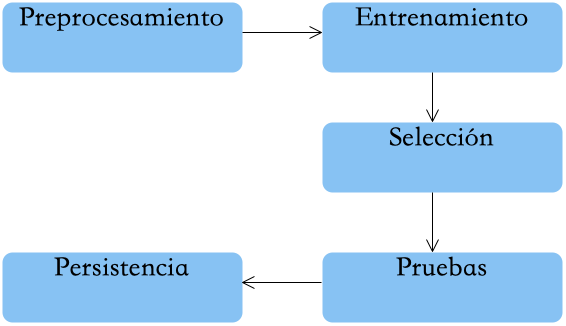
\includegraphics[scale=.55]{imagenes/capitulo5/Esquema.png}
\caption{Proceso de entrenamiento}
\label{fig:cp5:procesoE}
\end{figure}


%------------------------------------------------------------------%
\subsection{Preprocesamiento}

Como primera instancia, el corpus creado de 3500 noticias debe ser procesado, con el fin de crear vectores que representan el contenido de cada artículo de forma ordenada(ver ), de esta manera los algoritmos de clasificación son capaces de entender la información. En cuanto a los datos que son procesados de la noticia cabe mencionar que solo se usa el título y la redacción del artículo, los demás datos( como url, fecha, sección) no son necesarios para el entrenamiento. Este proceso consta de 6 etapas, las cuales son mostradas en la Figura \ref{fig:cp5:preprocesamiento}. \\

Cabe destacar que estas etapas están desarrolladas en un script escrito en el lenguaje \textbf{python 3}, en cada sección se hará mención de las librerías ocupadas.\\

\begin{figure}[h]
\centering
\includegraphics[scale=.55]{imagenes/capitulo5/preprocesamiento.png}
\caption{Etapas de preprocesamiento}
\label{fig:cp5:preprocesamiento}
\end{figure}

%----------------------------------%
\begin{large}
\textbf{Limpieza}\\
\end{large}

Esta etapa consiste en eliminar texto que no brinda información útil para el entrenamiento como, hipertexto (ver ), símbolos especiales (como \# $\dagger$ $\sqrt{ }$), \textit{emojis} (como \dSmiley \dCooley \dNinja). Por ejemplo el texto \ref{box:cp5:texto} muestra la redacción de una noticia con la información descargada de una pagina web. El resultado de limpiar la noticia se muestra en el texto \ref{box:cp5:limpio}. Se puede observar que se han eliminado los elementos $<p>\ </p>\ <!--\ -->$ \# $\dagger$ \dSmiley \dCooley \dInnocey.\\

Para realizar esta tarea se han ocupando las librerías; \textbf{pandas} (ver ) como medio de lectura de archivos tipo \textbf{CSV} (\textit{comma separeted values}, por sus siglas en ingles); \textbf{re} (ver ) la cual permite evaluar expresiones regulares con el objetivo de eliminar símbolos; \textbf{demoji} (ver ) quien permite eliminar \textit{emojis} dentro del texto.\\

\begin{mygraybox}[label={box:cp5:texto}]{Texto de entrada} 
$<p>\dagger$$\ \ \ $ El número 343 de El Trimestre Económico,$\otimes$ revista emblemática del Fondo de Cultura 
$<!--\ -->$
Económica (FCE), será * * * presentado por David Ibarra Muñoz \dSmiley , Carlos Tello Macías \dCooley , Alicia Puyana \dInnocey y Pablo Ruiz Nápoles el martes 27 de agosto a las 6 de la tarde, en la librería Rosario Castellanos, ubicada en avenida Tamaulipas \# 202, en la colonia Condesa de la capital mexicana.$</p>$
\end{mygraybox}

\ \\

\begin{mygraybox}[label={box:cp5:limpio}]{Texto limpio} 
El número 343 de El Trimestre Económico, revista emblemática del Fondo de Cultura 
Económica (FCE), será presentado por David Ibarra Muñoz, Carlos Tello Macías , Alicia Puyana y Pablo Ruiz Nápoles el martes 27 de agosto a las 6 de la tarde, en la librería Rosario Castellanos, ubicada en avenida Tamaulipas 202, en la colonia Condesa de la capital mexicana.
\end{mygraybox}
\ \\

%----------------------------------%
\begin{large}
\textbf{Filtro de longitud}\\
\end{large}

Con base en la regla de negocio (ver ) se ha definido 180 palabras como longitud mínima de las noticias, incluyendo en la definición de palabra números, signos de puntuación y exclamación.
Para esto después de haber concluido el proceso de limpieza se pregunta por la longitud de la cadena (sin contar los espacios) y si esta es mayor o igual a 180, entonces es un artículo válido para utilizar en el entrenamiento de lo contrario no es tomado en cuenta.\\

%----------------------------------%
\begin{large}
\textbf{Tokenizar}\\
\end{large}

La etapa de tokenización consiste en separar el texto en sus elementos mínimos llamados tokens, donde se separan palabras, signos de puntuación, llaves y números mediante un espacio. Continuando con el ejemplo \ref{box:cp5:limpio} donde el texto se encuentra limpio, se procede a su tokenización. El resultado es mostrado en el Cuadro \ref{box:cp5:tokenizar}. Para remarcar el ejemplo observe la palabra entre paréntesis \textbf{(FCE)} la cual es separada en \textbf{( FCE )} mostrando que ahora cada elemento representa un token individual. Para el desarrollo de esta tarea se ocupo la librería \textbf{RegexpTokenizer}.\\

\begin{mygraybox}[label={box:cp5:tokenizar}]{Texto tokenizado} 
El número 343 de El Trimestre Económico , revista emblemática del Fondo de Cultura 
Económica ( FCE ) , será presentado por David Ibarra Muñoz , Carlos Tello Macías , Alicia Puyana y Pablo Ruiz Nápoles el martes 27 de agosto a las 6 de la tarde , en la librería Rosario Castellanos , ubicada en avenida Tamaulipas 202 , en la colonia Condesa de la capital mexicana .
\end{mygraybox}
\ \\
%----------------------------------%
\begin{large}
\textbf{Lematizar}\\
\end{large}

Lematizar es el proceso de reducir cada palabra a su lemma, con el fin de eliminar ruido en el texto, por ejemplo las palabras correrás, corriendo, corrí, tienen como lema el verbo correr, el plural niños tiene como lema niño (ver ). Para realizar esta tarea se ha usado \textbf{spacy} (ver ) el cual es una librería de código abierto, con el diccionario \textit{es\_core\_news\_sm} quien permite analizar el léxico del lenguaje español.\\

Siguiendo con las etapas del proceso se toma el texto \ref{box:cp5:tokenizar} como entrada al programa y este da como salida el texto que se muestra en el Cuadro \ref{box:cp5:lematizado}.\\

\begin{mygraybox}[label={box:cp5:lematizado}]{Texto lematizado} 
el número 343 de el trimestre económico , revista emblemático del fondo de cultura económica ( fce ) , ser presentar por david ibarra muñoz , carlos tello macías , alicia puyana y pablo ruiz nápoles el martes 27 de agostar a los 6 de lo tardar , en lo librería rosario castellanos , ubicar en avenir tamaulipas 202 , en lo colonia condesa de lo capital mexicano .
\end{mygraybox}
\ \\

Cuando el proceso de lematización concluye se genera un identificador único para cada noticia el cual se define de la siguiente forma 

\begin{equation*}
id=<Identificador\ de\ sitio\ web><Numero\ de\ noticias>
\end{equation*}
 
donde \textbf{Identificador de sitio web} define un número único para hacer referencia a los sitios web (ver Tabla \ref{tab:cp5:sitioweb}) y  \textbf{Número de noticias} es el número del artículo.

\begin{table}[h]
\centering
	\begin{tabular}{|l|l|}
	%-----------------------Ecanbezado-----------------------------------%
		\hline
		\multicolumn{1}{| >{\columncolor{white!30!black}}l|}{ \textcolor{myWhite}{\textbf{Número}} }&
		\multicolumn{1}{| >{\columncolor{white!30!black}}l|}{ \textcolor{myWhite}{\textbf{Página web}} }\\
		\hline
	%------------------------------------------------%

		\textbf{100} & Aristegui noticias\\
		\hline
		\textbf{200} & Tv azteca\\
		\hline

		\textbf{300} & El Economista\\
		\hline

		\textbf{400} & La jornada\\	
		\hline

		\textbf{500} & La prensa\\
		\hline

		\textbf{600} & Proceso\\
		\hline

		\textbf{700} & Sopitas\\
		\hline

	\end{tabular}\\
\caption{Identificador de sito web}
\label{tab:cp5:sitioweb}
\end{table}


Como segundo paso las noticias son almacenadas en un archivo con extensión \textbf{TXT}, los elementos por almacenar son \textbf{id}, \textbf{titulo}, \textbf{noticia} y \textbf{sección}, los cuales son separados por los caracteres \&\&\&\&\& . El Cuadro \ref{box:cp5:archivo} muestra un ejemplo de la estructura del archivo.\\

\begin{mygraybox}[label={box:cp5:archivo}]{Estructura de archivo} 
id\&\&\&\&\&titulo\&\&\&\&\&noticia\&\&\&\&\&seccion\\
1001\&\&\&\&\&Titulo 1\&\&\&\&\&Contenido noticia 1\&\&\&\&\&0\\
...\\
5003500\&\&\&\&\&Titulo 3500\&\&\&\&\&Contenido noticia 3500\&\&\&\&\&4
\end{mygraybox}

\ \\

%----------------------------------%

\begin{large}
\textbf{División del corpus}\\
\end{large}


Para el correcto diseño y evaluación del algoritmos se requiere dividir el corpus en dos conjuntos: \textbf{entrenamiento} y \textbf{prueba}, con un 90\% y 10\% del total del \textit{dataset} respectivamente. En cada grupo deben estar repartidas noticias de las 5 secciones definidas, sin embargo los artículos almacenados están ordenados de forma descendente como: \textbf{Deportes}, \textbf{Economía}, \textbf{Política}, \textbf{Cultura}, \textbf{Ciencia y tecnología}, para seleccionar deforma distribuida los datos se ha ocupado una técnica llamada \textit{Shuffle}.\\

\textit{Shuffle} consiste en brindar un arreglo con los identificadores de las noticias y un número ( nombrado usualmente como semilla ), quien generar un nuevo orden en los identificadores de acuerdo a los números pseudo aleatorios que retorna esta función, tomando este como el nueva orden de los textos en el archivo de almacenamiento. Para el desarrollo de esta etapa se ha utilizado la librería \textbf{Shuffle} (ver ) con una semilla de 5.\\

Para ilustrar un ejemplo, en el cuadro \ref{box:cp5:ids} se muestra un conjunto de identificadores ordenados por el último número del $id$, al utilizar la función \textit{Shuffle} con una semilla de 2, se genera un nuevo orden el cual es mostrado en el Cuadro \ref{box:cp5:shuffle}.\\


\begin{mygraybox}[label={box:cp5:ids}]{Identificadores de noticias} 
\begin{equation*}
\begin{bmatrix}
1001 & 2002 & 3003 & 4004 & 5005 & 6006 & 7007 & 1008\\ 
\end{bmatrix}
\end{equation*}
\end{mygraybox}

\ \\


\begin{mygraybox}[label={box:cp5:shuffle}]{Nuevo orden de ID's} 
\begin{equation*}
\begin{bmatrix}
5005 & 2002 & 7007 & 3003 & 4004 & 1008 & 6006 & 1001\\
\end{bmatrix}
\end{equation*}
\end{mygraybox}
\ \\

La distribución generada por esta función es almacenada en un archivo, y como último paso se han tomado las primeras 350 noticias de forma manual y se han colocado en un archivo diferente, definido así las noticias de entrenamiento (con 3150) y de prueba (con 350).\\

La cantidad de noticias por sección del conjunto de entrenamiento se muestran en la Figura \ref{fig:cp5:seccionE} y del conjunto de prueba en la Figura \ref{fig:cp5:sitiosP}.



\begin{figure}[h]
\centering
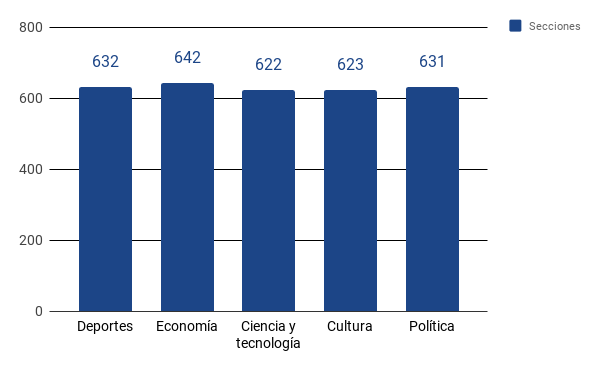
\includegraphics[scale=.6]{imagenes/capitulo5/SeccionesE.png}
\caption{Corpus de entrenamiento}
\label{fig:cp5:seccionE}
\end{figure}

\begin{figure}[H]
\centering
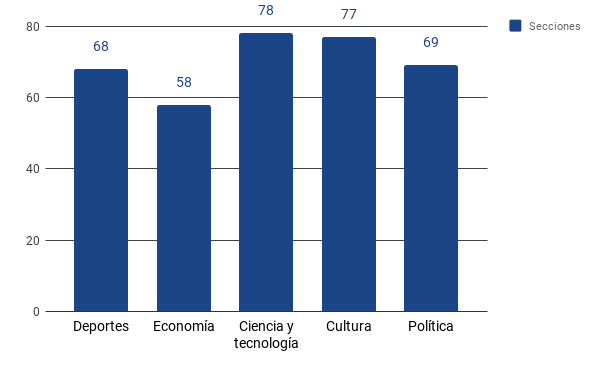
\includegraphics[scale=.6]{imagenes/capitulo5/SeccionesP.png}
\caption{Corpus de prueba}
\label{fig:cp5:seccionP}
\end{figure}

%\begin{figure}[h]
%\centering
%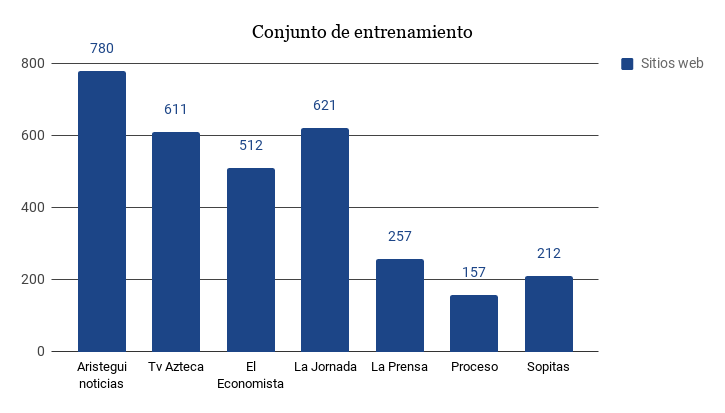
\includegraphics[scale=.6]{imagenes/capitulo5/SitiosE.png}
%\caption{Número de noticias pertenecientes a los sitios web}
%\label{fig:cp5:sitiosE}
%\end{figure}



%------------------------------------------------------------------%
\subsection{Entrenamiento}

Para crear un modelo clasificador ( el cual resuelve un problema multinomial ver ) usando aprendizaje supervisado (ver ), se debe construir dos conjuntos etiquetados: entrenamiento para el proceso de aprendizaje y otro de prueba, para medir su precisión. En la sección anterior estos grupos se han formado con noticias de 5 secciones: \textbf{Deportes}, \textbf{Economía}, \textbf{Política}, \textbf{Cultura}, \textbf{Ciencia y tecnología}. Ambos dataset serán usados en 4 algoritmos (seleccionados con base en el estado del arte ver ), los cuales son:

\begin{itemize}
	\item \textbf{Naive Bayes} (ver )
	\item \textbf{Regresión logística} (ver )
	\item \textbf{Maquina de soporte vectorial} (ver )
	\item \textbf{Random Forest} (ver )
\end{itemize}

El proceso de entrenamiento consta de 5 pasos los cuales se muestran en la Figura \ref{fig:cp5:entrenamiento}.

\begin{figure}[h]
\centering
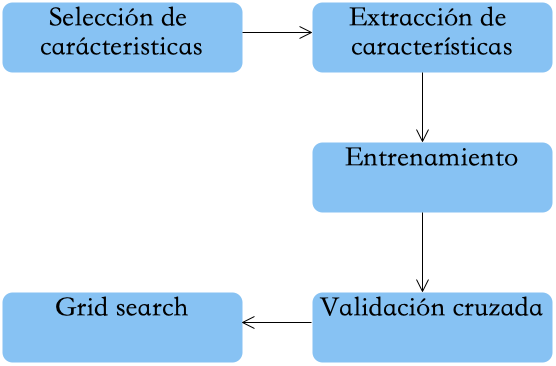
\includegraphics[scale=.5]{imagenes/capitulo5/Entrenamiento.png}
\caption{Etapas de entrenamiento}
\label{fig:cp5:entrenamiento}
\end{figure}

El desarrollo se ha implementado en el lenguaje de programación \textbf{Python 3}, ocupando la librería \textbf{scikit learn} quien permite crear instancias de los algoritmos mencionados. Cabe señalar que el objetivo de este trabajo terminal es el entrenamiento de los clasificadores y no su desarrollo.

Como primer paso del entrenamiento, el corpus debe ser traducido del lenguaje español a un conjunto de vectores numéricos que representan la información de las noticias, esta es llamada representación vectorial (ver ). Para lograr este objetivo, del \textit{dataset} se deben seleccionar características que definan los elementos del vector numérico.\\

%----------------------------------%
\begin{large}
\textbf{Selección de características}\\
\end{large}

Cada clase de noticias contiene un conjunto de palabras que son comunes en su ámbito, al analizar el léxico usado se observa los tecnicismos usados, por ejemplo ; en la sección deportes se ocupa, fútbol, jugador, ganador ; en política, presidente, corrupción, PRI ; en ciencia y tecnología, investigación, descubrimiento, publicación y así sucesivamente, por lo tanto estos vocablos pueden ser definidos como características que identifican a una sección. En este sentido la selección de características es el proceso de tomar el corpus de noticias e identificar las palabras mas comunes en los artículos.\\ 

Para ejemplificar esta tarea observe el Cuadro \ref{box:cp5:corpus} el cual es un corpus de 4 oraciones. Una vez realizado el proceso de extracción de características se obtiene las palabras relevantes las cuales son mostradas en el Cuadro \ref{box:cp5:caracteristicas}.\\

\begin{mygraybox}[label={box:cp5:corpus}]{Corpus} 
\begin{equation*}
\begin{bmatrix}
Este&es&la&primera&noticia\\
Esta&noticia&es&la&segunda&noticia\\
Y&este&es&la&tercera\\
Es&este&la&primera&noticia&?
\end{bmatrix}
\end{equation*}
\end{mygraybox}

\begin{mygraybox}[label={box:cp5:caracteristicas}]{Selección de características} 
\begin{equation*}
\begin{bmatrix}
es & esta & este & la & noticia & primera & segunda & tercera
\end{bmatrix}
\end{equation*}
\end{mygraybox}

%----------------------------------%

\ \\

\begin{large}
\textbf{Extracción de características}\\
\end{large}

Después de seleccionar las características, se crea un espacio vectorial por cada noticia donde cada elemento del vector representa la presencia o ausencia de una característica (palabra). Cabe mencionar que las características son extraídas de 2 formas, binario(donde 1 representa la presencia de la característica y 0 la ausencia) y por frecuencia ( donde se cuenta el número de veces que cada característica aparece). Continuando con el ejemplo del Cuadro \ref{box:cp5:corpus} se extraen las características por frecuencia y el resultado se muestra en el Cuadro \ref{box:cp5:frecuencia}, mientras que el Cuadro \ref{box:cp5:binario} muestra las características extraídas de forma binaria.\\

Para el desarrollo de esta etapa se ha implementado la librería \textbf{CountVectorizer} quien permite generar la selección y extracción de características. Cabe destacar que esta es la presentación vectorial (de cada noticia) que los algoritmos de clasificación pueden entender y por ende ser entrenados.\\

\begin{mygraybox}[label={box:cp5:frecuencia}]{Extracción por frecuencia} 
\begin{equation*}
\begin{bmatrix}
1 & 0 & 1 & 1 & 1 & 1 & 0 & 0\\ 
1 & 1 & 0 & 1 & 2 & 0 & 1 & 0\\
1 & 0 & 1 & 1 & 1 & 0 & 0 & 1\\
1 & 0 & 1 & 1 & 1 & 1 & 0 & 0\\
\end{bmatrix}
\end{equation*}
\end{mygraybox}

\ \\

\begin{mygraybox}[label={box:cp5:binario}]{Extracción binaría} 
\begin{equation*}
\begin{bmatrix}
1 & 0 & 1 & 1 & 1 & 1 & 0 & 0\\
1 & 1 & 0 & 1 & 1 & 0 & 1 & 0\\
1 & 0 & 1 & 1 & 1 & 0 & 0 & 1\\
1 & 0 & 1 & 1 & 1 & 1 & 0 & 0 
\end{bmatrix}
\end{equation*}
\end{mygraybox}

\ \\
%----------------------------------%

\begin{large}
\textbf{Entrenamiento}\\
\end{large}


El corpus contiene noticias de varias fuentes, en  las cuales la redacción, coherencia, semántica varía, incluso en la edición de una misma noticia, por lo tanto en el entrenamiento se busca generalizar la clasificación de los artículos, analizando el texto como un conjunto de palabras, sin tomar en cuenta la semántica, esta técnica es llamada bolsa de palabras (ver ).\\

En este punto del trabajo las noticias están representadas en un espacio vectorial, y serán usadas en el proceso de entrenamiento de los algoritmos: \textbf{Naive Bayes}, \textbf{Regresión logística}, \textbf{Maquina de soporte vectorial}, \textbf{Random Forest}. Cada clasificador reciben como entrada un conjunto de vectores etiquetados y como salida se genera un modelo el cual predice la sección de nuevos textos.\\ 

Para este trabajo se han definido las etiquetas como se muestra en la Tabla \ref{tab:cp5:etiquetas}, esta correspondencia es de secciones de noticias a un un número único.


\begin{table}[h]
\centering
	\begin{tabular}{|l|l|}
	%-----------------------Ecanbezado-----------------------------------%
		\hline
		\multicolumn{1}{| >{\columncolor{white!30!black}}l|}{ \textcolor{myWhite}{\textbf{Sección}} }&
		\multicolumn{1}{| >{\columncolor{white!30!black}}l|}{ \textcolor{myWhite}{\textbf{Etiqueta}} }\\
		\hline
	%------------------------------------------------%

		\textbf{Deportes} & 0 \\
		\hline

		\textbf{Economía} & 1 \\
		\hline
		\textbf{Política} & 2 \\
		\hline

		\textbf{Cultura} & 3 \\
		\hline

		\textbf{Ciencia y tecnología} & 4 \\	
		\hline

	\end{tabular}\\
\caption{Etiquetas de secciones}
\label{tab:cp5:etiquetas}
\end{table}


El desarrollo ha ocupado una instancia de cada algoritmo, para esto se incluye la librería correspondiente de \textbf{sciktlearn}, las cuales se muestran en la Tabla \ref{tab:cp5:librerias}, la entrada al clasificador es el conjunto de espacio vectorial y las etiquetas correspondientes, esto regresa como resultado un modelo que es capas de predecir la sección de noticias, sin que estas estén etiquetadas.

\begin{table}[h]
\centering
	\begin{tabular}{|l|l|}
	%-----------------------Ecanbezado-----------------------------------%
		\hline
		\multicolumn{1}{| >{\columncolor{white!30!black}}l|}{ \textcolor{myWhite}{\textbf{Sección}} }&
		\multicolumn{1}{| >{\columncolor{white!30!black}}l|}{ \textcolor{myWhite}{\textbf{Etiqueta}} }\\
		\hline
	%------------------------------------------------%

		\textbf{Naive Bayes} & MultinomialNB \\
		\hline

		\textbf{Maquina de soporte vectorial} & SVC\\
		\hline

		\textbf{Regresión logísitica} &LogisticRegression\\
		\hline

		\textbf{Ramdon Forest} &  RandomForestClassifier\\
		\hline

	\end{tabular}\\
\caption{Librería de algoritmo}
\label{tab:cp5:librerias}
\end{table}


%----------------------------------%

\begin{large}
\textbf{Validación cruzada}\\
\end{large}

%----------------------------------%

\begin{large}
\textbf{Grid search}\\
\end{large}


\begin{table}[H]
\centering
\resizebox{\columnwidth}{!}{%
	\begin{tabular}{|l|l|l|l|l|l|l|l|}
	%-----------------------Ecanbezado-----------------------------------%
		\hline
\multicolumn{1}{| >{\columncolor{myBlueChapter}}l|}{ \textcolor{myWhite}{\textbf{Parámetros}} }&
\multicolumn{1}{| >{\columncolor{myBlueChapter}}l|}{ \textcolor{myWhite}{\textbf{P 1}} }&
\multicolumn{1}{| >{\columncolor{myBlueChapter}}l|}{ \textcolor{myWhite}{\textbf{P 2}} }&
\multicolumn{1}{| >{\columncolor{myBlueChapter}}l|}{ \textcolor{myWhite}{\textbf{P 3}} }&
\multicolumn{1}{| >{\columncolor{myBlueChapter}}l|}{ \textcolor{myWhite}{\textbf{P 4}} }&
\multicolumn{1}{| >{\columncolor{myBlueChapter}}l|}{ \textcolor{myWhite}{\textbf{P 5}} }&
\multicolumn{1}{| >{\columncolor{myBlueChapter}}l|}{ \textcolor{myWhite}{\textbf{Promedio}} }&
\multicolumn{1}{| >{\columncolor{myBlueChapter}}l|}{ \textcolor{myWhite}{\textbf{Rank}} }
\\  \cline{1-8}
	%------------------------------------------------%
C: 100, gamma: 0.0001, kernel: rbf&0.8736&0.8639&0.8537&0.8726&0.8822&0.8692&1\\
\hline
C: 1000, gamma: 1e-05, kernel: rbf&0.8752&0.8623&0.8537&0.8710&0.8822&0.8689&2\\
\hline
C: 1000, gamma: 0.0001, kernel: rbf&0.8689&0.8608&0.8506&0.8694&0.8790&0.8657&3\\
\hline
C: 1, gamma: 0.0001, kernel: linear&0.8657&0.8592&0.8410&0.8710&0.8742&0.8622&4\\
\hline
C: 1, gamma: 1e-05, kernel: linear&0.8657&0.8592&0.8410&0.8710&0.8742&0.8622&4\\
\hline
C: 1, gamma: 1e-06, kernel: linear&0.8657&0.8592&0.8410&0.8710&0.8742&0.8622&4\\
\hline
C: 10, gamma: 0.0001, kernel: linear&0.8657&0.8592&0.8394&0.8710&0.8742&0.8619&5\\
\hline
C: 10, gamma: 1e-05, kernel: linear&0.8657&0.8592&0.8394&0.8710&0.8742&0.8619&5\\
\hline
C: 10, gamma: 1e-06, kernel: linear&0.8657&0.8592&0.8394&0.8710&0.8742&0.8619&5\\
\hline
C: 100, gamma: 0.0001, kernel: linear&0.8657&0.8592&0.8394&0.8710&0.8742&0.8619&5\\
\hline
C: 100, gamma: 1e-05, kernel: linear&0.8657&0.8592&0.8394&0.8710&0.8742&0.8619&5\\
\hline
C: 100, gamma: 1e-06, kernel: linear&0.8657&0.8592&0.8394&0.8710&0.8742&0.8619&5\\
\hline
C: 1000, gamma: 0.0001, kernel: linear&0.8657&0.8592&0.8394&0.8710&0.8742&0.8619&5\\
\hline
C: 1000, gamma: 1e-05, kernel: linear&0.8657&0.8592&0.8394&0.8710&0.8742&0.8619&5\\
\hline
C: 1000, gamma: 1e-06, kernel: linear&0.8657&0.8592&0.8394&0.8710&0.8742&0.8619&5\\
\hline
C: 10, gamma: 0.0001, kernel: rbf&0.8641&0.8576&0.8490&0.8678&0.8503&0.8578&6\\
\hline
C: 100, gamma: 1e-05, kernel: rbf&0.8641&0.8576&0.8490&0.8662&0.8519&0.8578&6\\
\hline
C: 1000, gamma: 1e-06, kernel: rbf&0.8641&0.8576&0.8490&0.8662&0.8519&0.8578&6\\
\hline
C: 100, gamma: 1e-06, kernel: rbf&0.6524&0.6772&0.6073&0.6449&0.6608&0.6485&7\\
\hline
C: 10, gamma: 1e-05, kernel: rbf&0.6493&0.6741&0.6073&0.6401&0.6561&0.6454&8\\
\hline
C: 1, gamma: 0.0001, kernel: rbf&0.6193&0.6440&0.5946&0.6115&0.6306&0.6200&9\\
\hline
C: 1, gamma: 0.0001, kernel: poly&0.2038&0.2041&0.2035&0.2038&0.2038&0.2038&10\\
\hline
C: 1, gamma: 1e-05, kernel: poly&0.2038&0.2041&0.2035&0.2038&0.2038&0.2038&10\\
\hline
C: 1, gamma: 1e-05, kernel: rbf&0.2038&0.2041&0.2035&0.2038&0.2038&0.2038&10\\
\hline
C: 1, gamma: 1e-06, kernel: poly&0.2038&0.2041&0.2035&0.2038&0.2038&0.2038&10\\
\hline
C: 1, gamma: 1e-06, kernel: rbf&0.2038&0.2041&0.2035&0.2038&0.2038&0.2038&10\\
\hline
C: 10, gamma: 0.0001, kernel: poly&0.2038&0.2041&0.2035&0.2038&0.2038&0.2038&10\\
\hline
C: 10, gamma: 1e-05, kernel: poly&0.2038&0.2041&0.2035&0.2038&0.2038&0.2038&10\\
\hline
C: 10, gamma: 1e-06, kernel: poly&0.2038&0.2041&0.2035&0.2038&0.2038&0.2038&10\\
\hline
C: 10, gamma: 1e-06, kernel: rbf&0.2038&0.2041&0.2035&0.2038&0.2038&0.2038&10\\
\hline
C: 100, gamma: 0.0001, kernel: poly&0.2038&0.2041&0.2035&0.2038&0.2038&0.2038&10\\
\hline
C: 100, gamma: 1e-05, kernel: poly&0.2038&0.2041&0.2035&0.2038&0.2038&0.2038&10\\
\hline
C: 100, gamma: 1e-06, kernel: poly&0.2038&0.2041&0.2035&0.2038&0.2038&0.2038&10\\
\hline
C: 1000, gamma: 0.0001, kernel: poly&0.2038&0.2041&0.2035&0.2038&0.2038&0.2038&10\\
\hline
C: 1000, gamma: 1e-05, kernel: poly&0.2038&0.2041&0.2035&0.2038&0.2038&0.2038&10\\
\hline
C: 1000, gamma: 1e-06, kernel: poly&0.2038&0.2041&0.2035&0.2038&0.2038&0.2038&10\\
\hline

	\end{tabular}
}
\caption{Maquina de soporte vectorial}
\label{tab:cp5:msv}
\end{table}




\begin{table}[H]
\centering
\resizebox{\columnwidth}{!}{%
	\begin{tabular}{|l|l|l|l|l|l|l|l|}
	%-----------------------Ecanbezado-----------------------------------%
		\hline
\multicolumn{1}{| >{\columncolor{myBlueChapter}}l|}{ \textcolor{myWhite}{\textbf{Parámetros}} }&
\multicolumn{1}{| >{\columncolor{myBlueChapter}}l|}{ \textcolor{myWhite}{\textbf{P 1}} }&
\multicolumn{1}{| >{\columncolor{myBlueChapter}}l|}{ \textcolor{myWhite}{\textbf{P 2}} }&
\multicolumn{1}{| >{\columncolor{myBlueChapter}}l|}{ \textcolor{myWhite}{\textbf{P 3}} }&
\multicolumn{1}{| >{\columncolor{myBlueChapter}}l|}{ \textcolor{myWhite}{\textbf{P 4}} }&
\multicolumn{1}{| >{\columncolor{myBlueChapter}}l|}{ \textcolor{myWhite}{\textbf{P 5}} }&
\multicolumn{1}{| >{\columncolor{myBlueChapter}}l|}{ \textcolor{myWhite}{\textbf{Promedio}} }&
\multicolumn{1}{| >{\columncolor{myBlueChapter}}l|}{ \textcolor{myWhite}{\textbf{Rank}} }
\\  \cline{1-8}
	%--------------
C: 0.1, penalty: l2, solver: liblinear&0.8768&0.8655&0.8521&0.8710&0.8758&0.8682&1\\
\hline
C: 0.01, penalty: l2, solver: liblinear&0.8705&0.8655&0.8474&0.8742&0.8615&0.8638&2\\
\hline
C: 0.1, penalty: l1, solver: liblinear&0.8515&0.8544&0.8442&0.8424&0.8376&0.8460&3\\
\hline
C: 0.001, penalty: l2, solver: liblinear&0.8436&0.8560&0.8299&0.8392&0.8169&0.8371&4\\
\hline
C: 0.0001, penalty: l2, solver: liblinear&0.7836&0.7832&0.7806&0.7739&0.7723&0.7787&5\\
\hline
C: 0.01, penalty: l1, solver: liblinear&0.6477&0.6297&0.5946&0.6099&0.6099&0.6184&6\\
\hline
C: 1e-05, penalty: l2, solver: liblinear&0.6051&0.6044&0.6057&0.5924&0.5796&0.5974&7\\
\hline
C: 1e-06, penalty: l2, solver: liblinear&0.5261&0.5316&0.5564&0.5223&0.5048&0.5282&8\\
\hline
C: 1e-06, penalty: l1, solver: liblinear&0.2006&0.2009&0.2003&0.2006&0.2006&0.2006&9\\
\hline
C: 1e-05, penalty: l1, solver: liblinear&0.2006&0.2009&0.2003&0.2006&0.2006&0.2006&9\\
\hline
C: 0.0001, penalty: l1, solver: liblinear&0.2006&0.2009&0.2003&0.2006&0.2006&0.2006&9\\
\hline
C: 0.001, penalty: l1, solver: liblinear&0.2006&0.2009&0.2003&0.2006&0.2006&0.2006&9\\
\hline
	\end{tabular}
}
\caption{Regresión logística}
\label{tab:cp5:regresion}
\end{table}


\begin{table}[H]
\centering
\resizebox{\columnwidth}{!}{%
	\begin{tabular}{|l|l|l|l|l|l|l|l|}
	%-----------------------Ecanbezado-----------------------------------%
		\hline
\multicolumn{1}{| >{\columncolor{myBlueChapter}}l|}{ \textcolor{myWhite}{\textbf{Parámetros}} }&
\multicolumn{1}{| >{\columncolor{myBlueChapter}}l|}{ \textcolor{myWhite}{\textbf{P 1}} }&
\multicolumn{1}{| >{\columncolor{myBlueChapter}}l|}{ \textcolor{myWhite}{\textbf{P 2}} }&
\multicolumn{1}{| >{\columncolor{myBlueChapter}}l|}{ \textcolor{myWhite}{\textbf{P 3}} }&
\multicolumn{1}{| >{\columncolor{myBlueChapter}}l|}{ \textcolor{myWhite}{\textbf{P 4}} }&
\multicolumn{1}{| >{\columncolor{myBlueChapter}}l|}{ \textcolor{myWhite}{\textbf{P 5}} }&
\multicolumn{1}{| >{\columncolor{myBlueChapter}}l|}{ \textcolor{myWhite}{\textbf{Promedio}} }&
\multicolumn{1}{| >{\columncolor{myBlueChapter}}l|}{ \textcolor{myWhite}{\textbf{Rank}} }
\\  \cline{1-8}
	%--------------
max\_depth: 50, n\_estimators: 1000&0.8720&0.8592&0.8537&0.8631&0.8615&0.8619&1\\
\hline
max\_depth: 1000, n\_estimators: 1000&0.8689&0.8639&0.8585&0.8583&0.8583&0.8616&2\\
\hline
max\_depth: 100, n\_estimators: 1000&0.8752&0.8592&0.8569&0.8599&0.8551&0.8613&3\\
\hline
max\_depth: 100, n\_estimators: 500&0.8784&0.8608&0.8601&0.8535&0.8519&0.8609&4\\
\hline
max\_depth: 1000, n\_estimators: 500&0.8720&0.8528&0.8585&0.8551&0.8599&0.8597&5\\
\hline
max\_depth: 50, n\_estimators: 500&0.8705&0.8544&0.8601&0.8535&0.8599&0.8597&6\\
\hline
max\_depth: 500, n\_estimators: 1000&0.8720&0.8655&0.8506&0.8487&0.8583&0.8590&7\\
\hline
max\_depth: 500, n\_estimators: 500&0.8689&0.8544&0.8553&0.8519&0.8615&0.8584&8\\
\hline
max\_depth: 500, n\_estimators: 100&0.8610&0.8608&0.8506&0.8487&0.8662&0.8575&9\\
\hline
max\_depth: 50, n\_estimators: 100&0.8641&0.8528&0.8601&0.8503&0.8455&0.8546&10\\
\hline
max\_depth: 1000, n\_estimators: 100&0.8594&0.8528&0.8474&0.8392&0.8439&0.8485&11\\
\hline
max\_depth: 100, n\_estimators: 100&0.8657&0.8560&0.8394&0.8471&0.8280&0.8473&12\\
\hline
max\_depth: 50, n\_estimators: 50&0.8626&0.8402&0.8267&0.8583&0.8471&0.8470&13\\
\hline
max\_depth: 100, n\_estimators: 50&0.8420&0.8402&0.8283&0.8503&0.8535&0.8429&14\\
\hline
max\_depth: 500, n\_estimators: 50&0.8531&0.8418&0.8331&0.8424&0.8312&0.8403&15\\
\hline
max\_depth: 1000, n\_estimators: 50&0.8578&0.8212&0.8315&0.8392&0.8280&0.8355&16\\
\hline
	\end{tabular}
}
\caption{Random Forest}
\label{tab:cp5:random}
\end{table}


\begin{table}[H]
\centering
\resizebox{\columnwidth}{!}{%
	\begin{tabular}{|l|l|l|l|l|l|l|l|}
	%-----------------------Ecanbezado-----------------------------------%
		\hline
\multicolumn{1}{| >{\columncolor{myBlueChapter}}l|}{ \textcolor{myWhite}{\textbf{Parámetros}} }&
\multicolumn{1}{| >{\columncolor{myBlueChapter}}l|}{ \textcolor{myWhite}{\textbf{P 1}} }&
\multicolumn{1}{| >{\columncolor{myBlueChapter}}l|}{ \textcolor{myWhite}{\textbf{P 2}} }&
\multicolumn{1}{| >{\columncolor{myBlueChapter}}l|}{ \textcolor{myWhite}{\textbf{P 3}} }&
\multicolumn{1}{| >{\columncolor{myBlueChapter}}l|}{ \textcolor{myWhite}{\textbf{P 4}} }&
\multicolumn{1}{| >{\columncolor{myBlueChapter}}l|}{ \textcolor{myWhite}{\textbf{P 5}} }&
\multicolumn{1}{| >{\columncolor{myBlueChapter}}l|}{ \textcolor{myWhite}{\textbf{Promedio}} }&
\multicolumn{1}{| >{\columncolor{myBlueChapter}}l|}{ \textcolor{myWhite}{\textbf{Rank}} }
\\  \cline{1-8}
	%--------------

alpha: 0.5&0.8610&0.8576&0.8458&0.8487&0.8424&0.8511&1\\
\hline
alpha: 1&0.8531&0.8497&0.8426&0.8408&0.8360&0.8444&2\\
\hline
alpha: 1.5&0.8531&0.8434&0.8410&0.8392&0.8312&0.8416&3\\
\hline
alpha: 2&0.8531&0.8418&0.8410&0.8392&0.8296&0.8409&4\\
\hline

	\end{tabular}
}
\caption{Naive bayes}
\label{tab:cp5:naive}
\end{table}



%------------------------------------------------------------------%
\subsection{Pruebas}
%------------------------------------------------------------------%
\subsection{Selección}
%------------------------------------------------------------------%
\subsection{Persistencia}

%\subsection{Tokenizar}
%\subsection{Lematizar}
%\subsection{Validación cruzada}
%\subsection{Shuffle}
%\subsection{Grid search}
%\subsection[Resultados]{Selección y resultado del mejor clasificador}
%\subsection[Persistencia]{Persistencia del clasificador}